\chapter{Idealised Section U --- Analytical vs.\ ANSYS}
\label{ch:assignment4}

\begingroup\itshape Assignment 4 --- 20 points\endgroup


\bigskip


\section{Analytical model vs.\ ANSYS model}
\label{sec:a4-1}

\begin{table}[h]
\begin{tabular}{|l|l|l|}
\hline
-                         & \textbf{value} & \textbf{unit} \\ \hline
\textbf{Length}           & 20000          & {[}mm{]}      \\ \hline
\textbf{width}            & 8000           & {[}mm{]}      \\ \hline
\textbf{density}          & 7,850          & {[}ton/m3{]}  \\ \hline
\textbf{Torsional moment} & 1000           & {[}Nmm{]}     \\ \hline
\textbf{Depth}            & 5000           & {[}mm{]}      \\ \hline
\textbf{Side thickness}   & 70             & {[}mm{]}      \\ \hline
\textbf{Bottom thickness} & 130            & {[}mm{]}      \\ \hline
\textbf{Youngs modulus (E)}   & 205000         & n/mm2         \\ \hline
\textbf{Shear modulus (G)}   & 81000         & n/mm2         \\ \hline
\textbf{Poisson ratio}    & 0.3            & {[}-{]}       \\ \hline
\textbf{Ip side}    &    $775.3a^5t_p$      &    mm^4  \\ \hline
\textbf{Ip bottom}    &    $387.7a^5t_p$    &    mm^4  \\ \hline
\end{tabular}
\end{table}

\paragraph{Modelling approach in ANSYS (common to all sub-questions).}
\begin{enumerate}[label=(\arabic*), leftmargin=*]
  \item \emph{Geometry}: \tbd{model, elementtype}
  \item \emph{Mesh}: \tbd{meshdichtheid en convergentiecheck}
  \item \emph{Free-warping load case}: \tbd{belasting en opleggingen}
  \item \emph{Constrained-warping load case}: \tbd{belasting en opleggingen}
  \item \emph{Post-processing}: \tbd{paden, uitvoer en export}
\end{enumerate}

\subsection{Free warping shear stress}
\label{sec:a4-a}


\begin{enumerate}[label=\roman*., leftmargin=*]
  \item 
\begin{align}
    \tau_{xs} &= G\left(\frac{\partial u}{\partial s} + \rho\theta\right) \\
    u &= \theta\,\omega(s) \rightarrow \frac{\partial u}{\partial s} = \theta \frac{\partial\omega}{\partial s} \\
    \theta &= \frac{M_t}{GI_p}
\end{align}

Then for each member, with e as the distance to the CoR:
\begin{align}
    u_{32} = &\frac{M_t}{GI_p}*\omega_{32} = \frac{M_t}{GI_p}*e*s\\
    u_{34} = &\frac{M_t}{GI_p}*\omega_{34} = \frac{M_t}{GI_p}*-e*s\\
     u_{21} = &\frac{M_t}{GI_p}*\omega_{21} = \frac{M_t}{GI_p} (B/2)(s-e)   \\
       u_{45} = &\frac{M_t}{GI_p}*\omega_{45} = \frac{M_t}{GI_p} (B/2)(-s+e) 
\end{align}
This gives the following stress equations, where in the side plating the $\tau_{xz}$ direction is important, and in the bottom plating the $\tau_{xy}$ direction.
\begin{align}
    \tau_{xz} &= \frac{M_t}{GI_p} *(B/2-B/2*t_p/2) \\
    \tau_{xz} &=  \frac{M_t}{GI_p}* (e-e*t_p/2)
\end{align}

        
  \item 
  The 2 images below show both the $\tau_{xy}$ and $\tau_{xz}$ respectively for the same idealized U section. Here one end has a completely fixed boundary condition and the other a free-rotating BC. Here the CW = 1. \textbf{CW moet 0 zijn want het is free warping. dus opnieuw plots maken. En analytical moet je de waardes uit de notepad in de formules van som 2 stampen.}


\begin{figure}[h]
    \centering
    \begin{minipage}{0.48\linewidth}
        \centering
        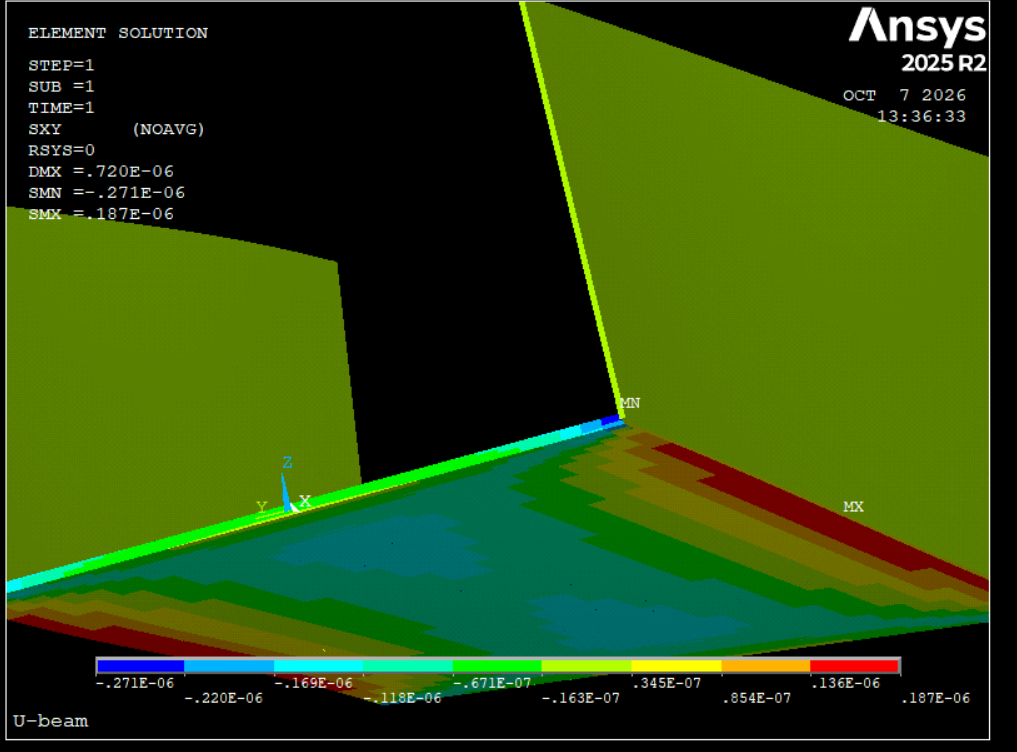
\includegraphics[width=\linewidth]{tauXY.png}
        \caption{TauXY shear stress in ANSYS model}
        \label{fig:tauXY}
    \end{minipage}
    \hfill
    \begin{minipage}{0.48\linewidth}
        \centering
        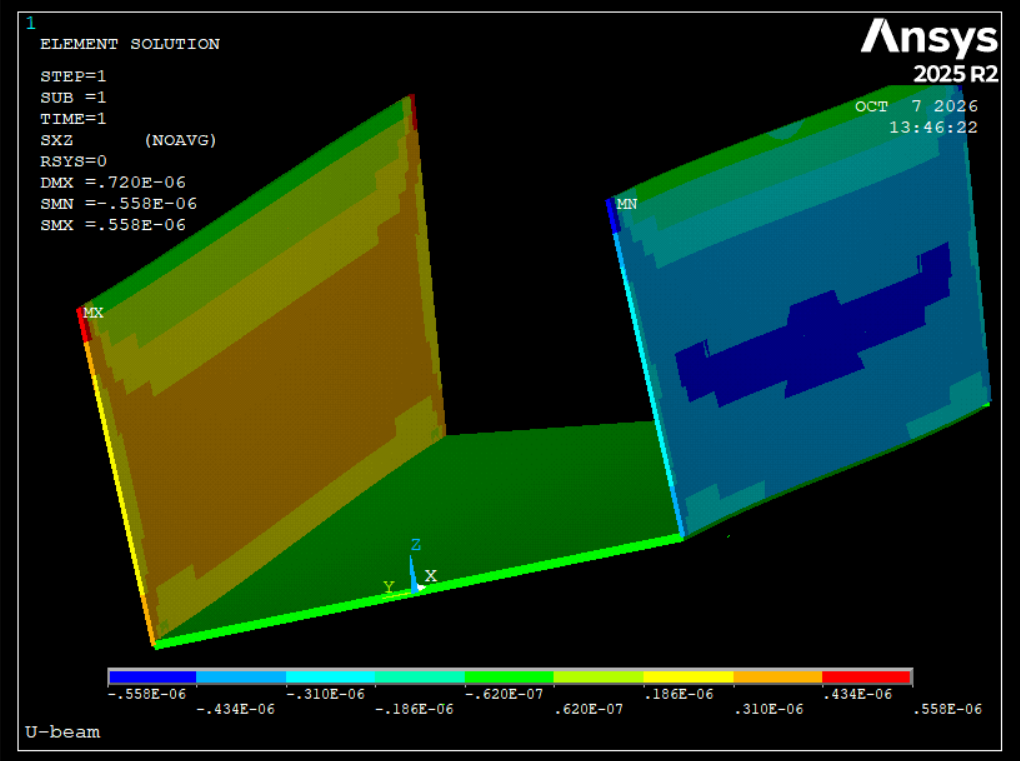
\includegraphics[width=\linewidth]{TauXZ.png}
        \caption{TauXZ shear stress in ANSYS model}
        \label{fig:tauXZ}
    \end{minipage}
\end{figure}

  \item Analytical and numerical solution in a single plot per component.
        \textbf{(1 pt)} \\ \tbd{overlay-plot}
  \item Discussion of the through-thickness distribution and maximum values.
        \textbf{(2 pts)} \\ \tbd{discussie}
\end{enumerate}

\subsection{Free warping displacement}
\label{sec:a4-b}

 
\begin{enumerate}[label=\roman*., leftmargin=*]
\item
Because the saection remains the same, the sectorial coordinates can remain the same as in the previous assignment.
\begin{align}
    u &= \theta*\omega(s)\\
    u_{32} = &\frac{M_t}{GI_p}*\omega_{32} = \frac{M_t}{GI_p}*z_ss\\
    u_{34} = &\frac{M_t}{GI_p}*\omega_{34} = \frac{M_t}{GI_p}*-z_ss\\
     u_{21} = &\frac{M_t}{GI_p}*\omega_{21} = \frac{M_t}{GI_p} (B/2)(s-z_s)   \\
  u_{45} = &\frac{M_t}{GI_p}*\omega_{45} = \frac{M_t}{GI_p} (B/2)(-s+z_s)     
\end{align}

  
  \item This section request specifically free warping displacement, thus CW is set to 0.

  \begin{figure}[h]
      \centering
      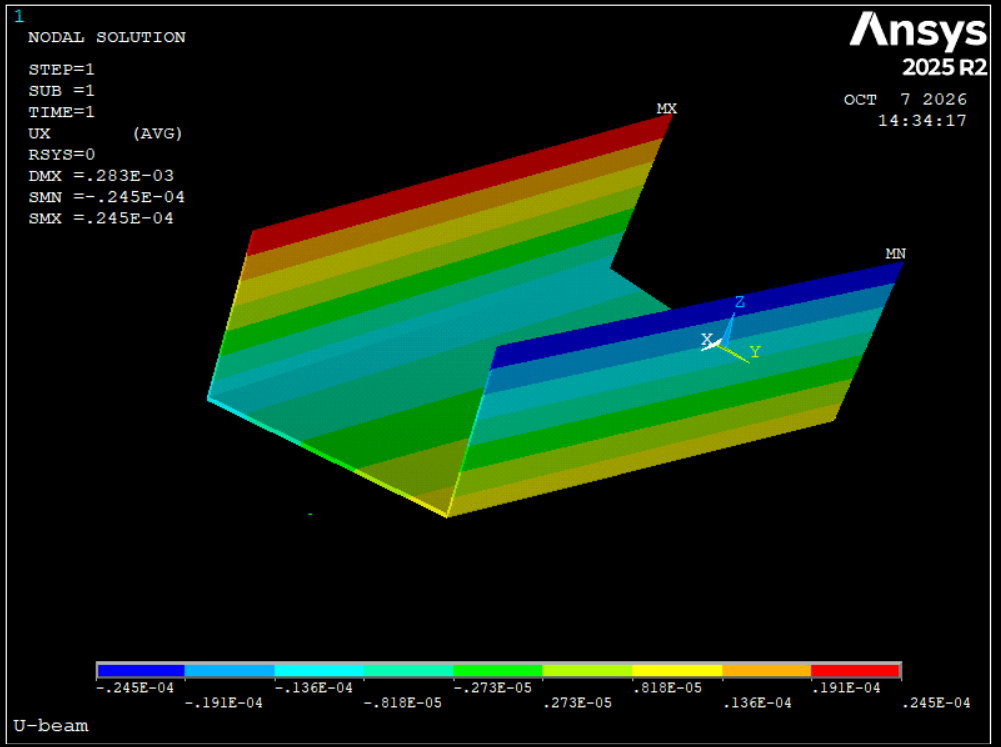
\includegraphics[width=0.5\linewidth]{X_displacement.png}
      \caption{u(s) in x direction is ANSYS model}
      \label{fig:placeholder}
  \end{figure}
        
  \item Overlay plot. \textbf{(1 pt)} \\ \tbd{overlay-plot}
  \item Discussion of the $s$-distribution and extreme values. \textbf{(2 pts)}
        \\ \tbd{discussie}
\end{enumerate}

\subsection{Constrained warping stress}
\label{sec:a4-c}
 Use $I_w$ obtained in
Assignment~2.6. \textbf{(5 pts)}

\begin{enumerate}[label=\roman*., leftmargin=*]
  \item Analytical $\sigma_{xx}(s) =E * \frac{d\theta}{dx} *\omega(s)$ \\



  
  \item ANSYS plot of $\sigma_{xx}(s)$ with settings. \textbf{(1 pt)}
        \\ \tbd{screenshot en instellingen}
  \item Overlay plot. \textbf{(1 pt)} \\ \tbd{overlay-plot}
  \item Discussion. \textbf{(2 pts)} \\ \tbd{discussie}
\end{enumerate}

\subsection{Constrained warping shear stress}
\label{sec:a4-d}

\questionbox{Calculate and compare the constrained warping shear stress
distribution $\tau_{xy}(s)$ and $\tau_{xz}(s)$. Use $S_\omega(s)$ obtained in
Assignment~2.5. \textbf{(5 pts)}}

\begin{enumerate}[label=\roman*., leftmargin=*]
  \item Analytical $\tau_{xy}(s)$, $\tau_{xz}(s)$. \textbf{(1 pt)}
        \\ \tbd{Uitwerking}
  \item ANSYS plot with settings. \textbf{(1 pt)}
        \\ \tbd{screenshot en instellingen}
  \item Overlay plot per component. \textbf{(1 pt)} \\ \tbd{overlay-plot}
  \item Discussion of through-thickness and $s$-distribution and maxima.
        \textbf{(2 pts)} \\ \tbd{discussie}
\end{enumerate}
